\documentclass[12pt]{article}
\usepackage{amsmath}
\usepackage{amsfonts}
\usepackage{geometry}
\usepackage{graphicx}
\usepackage{setspace}
\usepackage{parskip}
\usepackage{hyperref}
\usepackage{graphicx}
\usepackage{float}
\newcommand{\comm}[1]{def}

\geometry{a4paper, margin=1in}
\setstretch{1.2}

\title{\Huge Statistical Outlier Detection Notes}
\author{}
\date{}

\begin{document}

\maketitle

\section*{Outlier Detection Using Mean and Standard Deviation (Z-Score Based Outlier Detection)}

To detect outliers in a dataset $\Delta$, we use the mean and standard deviation:

\begin{itemize}
    \item $\mu(\Delta)$: Mean of the data
    \item $\sigma(\Delta)$: Standard deviation of the data
\end{itemize}

\subsection*{Normal Range}

The normal range is defined as:

\[
\mu(\Delta) \pm 2\sigma(\Delta)
\]

This means most data points (about 95\% if normally distributed) are expected to lie within this range.

\subsection*{Outlier Condition}

A value is considered an outlier if:

\[
\Delta < \mu(\Delta) - 2\sigma(\Delta) \quad \text{or} \quad \Delta > \mu(\Delta) + 2\sigma(\Delta)
\]



\begin{itemize}
    \item $\Delta$ - Orderbook Delta Depth of 5\% from Coinbase (BTC/USD) 
    \item $\mu(\Delta)$ - Mean of $\Delta$
    \item $\sigma(\Delta)$ - Standard deviation of the dataset
\end{itemize}


\subsection*{Lookahead Bias}




\subsection*{Strength of Signal}

To not only detect outlier price points but also see how far they are expanded from the mean I use the Z-score for each data point being detected as an outliers
\newpage
The Z-score is calculated as:

\[
Z = \frac{\Delta_5 - \mu(\Delta_5)}{\sigma(\Delta_5)}
\]

Only points outside the $[\mu - 2\sigma, \mu + 2\sigma]$ interval are considered outliers.  
For these, the signal strength is defined as $|Z|$, indicating how extreme the value is compared to the distribution.

\textit{Example:}  
A point with a Z-score of $+3.1$ is a stronger signal than one at $+2.1$, since it is farther from the mean.  
Non-outliers receive a signal strength of 0. 
\footnote{Visualisation inside of Figure 1}





\begin{figure}
    \centering
    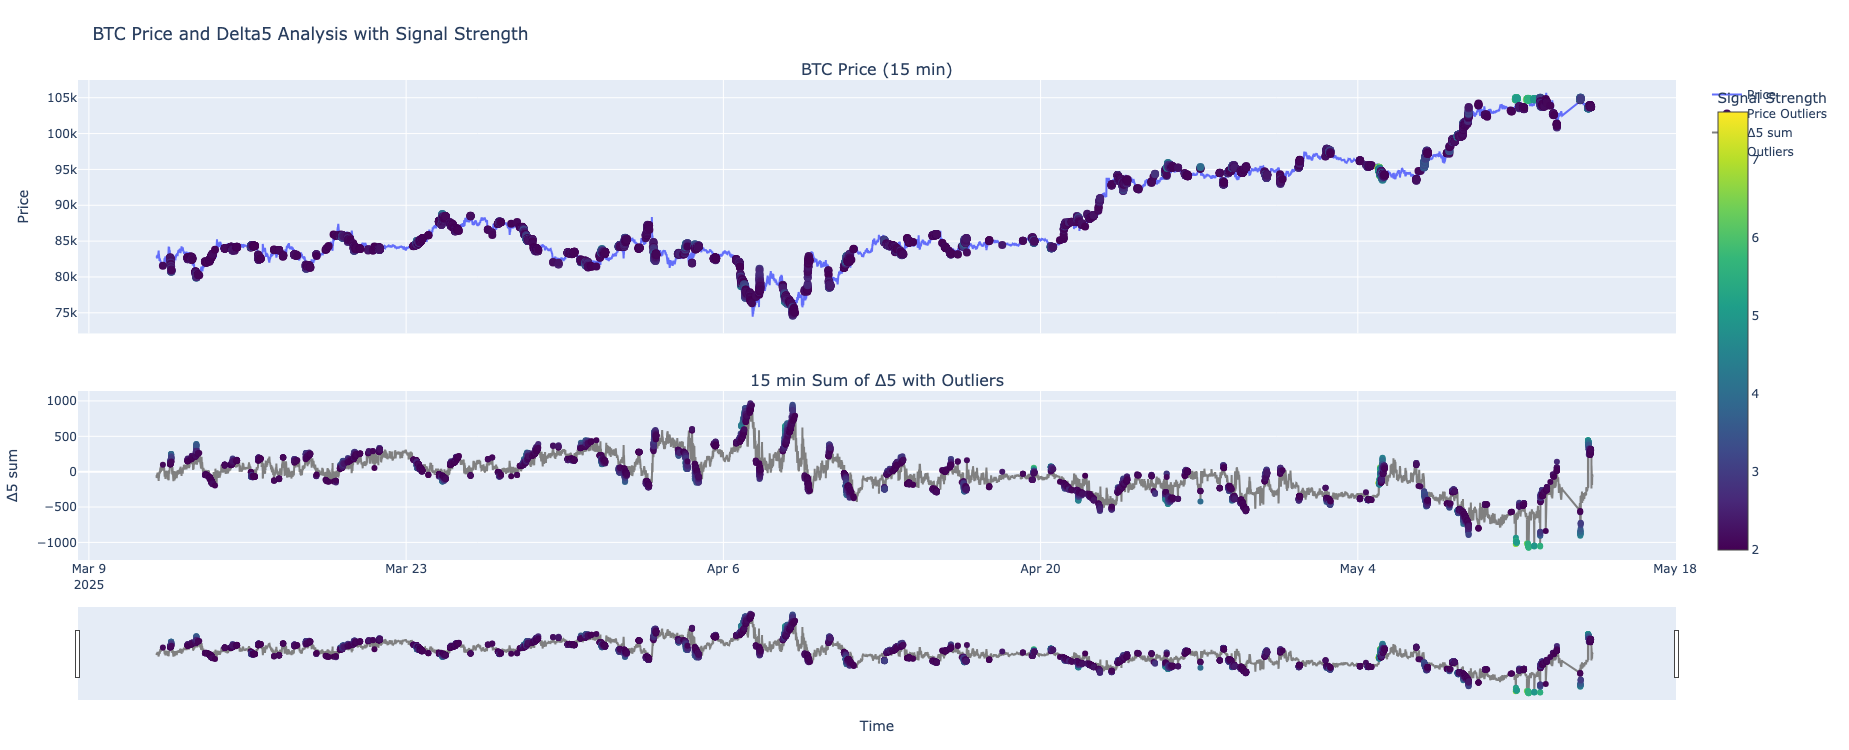
\includegraphics[width=1\textwidth]{imgs/outlier_signal_visualised.png}
    \caption{Heatmap Outlier}
\end{figure}




\newpage


\subsection*{Idea behind}

\begin{itemize}
    \item This method assumes data is roughly normally distributed.
    \item Using $2\sigma$ captures approximately 95\% of data points under a normal distribution.
    \item You can adjust the multiplier (e.g., $3\sigma$) for stricter or looser thresholds.
\end{itemize}





\subsection*{Future Plans}

\begin{itemize}
    \item Test on more data
    \item use rolling windows (e.g. 1 day or 1 week) for local context.
    \item Compare sensitivity with +- 1.5$\sigma$ or +-2.5$\sigma$
\end{itemize}

\newpage





\section*{Measuring Volatility After Price Outlier Detection}


\begin{equation}
    r_t = \frac{P_{t} - P_{t-1}}{P_{t-1}}
\end{equation}


\subsection*{Dictionary of Terms}

\begin{itemize}
    \item $P_t$  
      Asset price at time $t$.
    \item $r_t = \dfrac{P_t - P_{t-1}}{P_{t-1}}$  
      – 1-minute price return at time $t$.
    \item $\sigma^{\mathrm{(15)}}_{t}$  
      – Realized volatility: the standard deviation of the next 15 one-minute returns,
      \[
        \sigma^{\mathrm{(15)}}_{t}
        = \sqrt{\frac{1}{14}\sum_{i=1}^{15}\bigl(r_{t+i}-\bar r_{t}\bigr)^{2}},
        \quad
        \bar r_{t} = \frac{1}{15}\sum_{i=1}^{15} r_{t+i}
      \]
      aligned so that at time $t$ it measures volatility over $t+1$ to $t+15$.
\end{itemize}



\subsection*{In Py code}

\begin{verbatim}
import pandas as pd
df = pd.read_csv(file_path)
df.set_index('timestamp', inplace=True)
#Compute 1-min return of delta_5

df['r_t'] = df['price'].pct_change().fillna(0)


#compute rolling std of the future 15 min window

window = 15

#rolling on r_t, then shift forward so index t hold vol of t+1...t+15
df['future_vol_15] = (
    df['r_t']
    .rolling(window=window)
    .std()
    .shift(-window)
)






\end{verbatim}


\newpage

\section*{Combining Indicators}
Here I visulised the swing points, the EMA spread and the 100 outliers with the highest Z-Score in the same plot.

\begin{figure}[H]
    \centering
    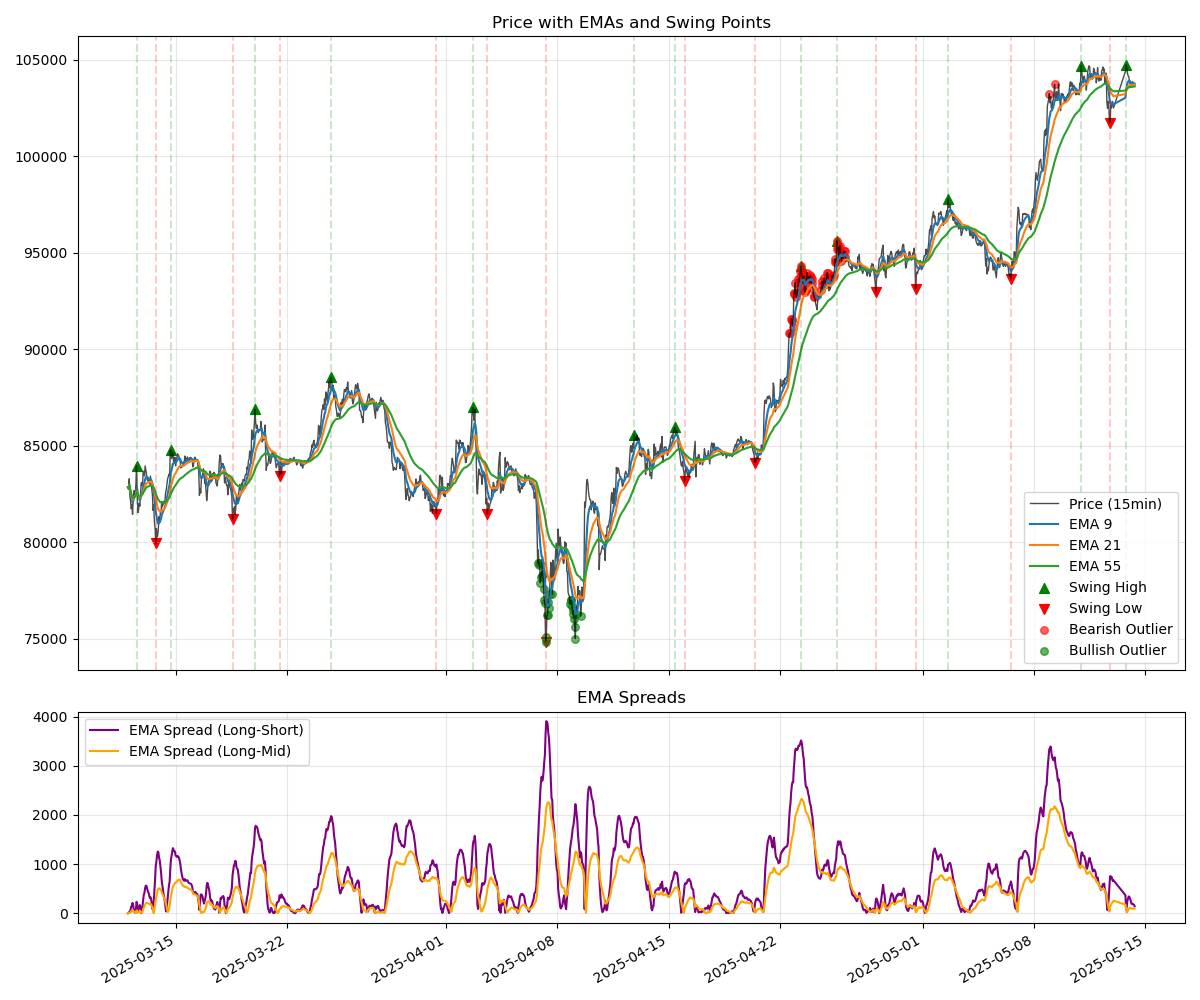
\includegraphics[width=\textwidth]{imgs/swingpoints_emaspread_priceOutliers.png}
    \caption{combined indicators png}
\end{figure}

\footnote{Chart made with Matplotlib and Seaborn}

\end{document}